\section{Luthfi Muhammad Nabil/1174035}
\subsection{Soal 1}
Buatlah fungsi pada file chap4\_1174035\_csv.py untuk membuka file csv dengan lib csv mode list : 
\lstinputlisting[firstline=2, lastline=6]{src/4/1174035/Praktek/chap4_1174035_csv.py}

\subsection{Soal 2}
Buatlah fungsi pada file chap4\_1174035\_csv.py untuk membuka file csv dengan lib csv mode dictionary : 
\lstinputlisting[firstline=8, lastline=12]{src/4/1174035/Praktek/chap4_1174035_csv.py}

\subsection{Soal 3}
Buatlah fungsi pada file chap4\_1174035\_pandas.py untuk membuka file csv dengan lib pandas mode list : 
\lstinputlisting[firstline=2, lastline=5]{src/4/1174035/Praktek/chap4_1174035_pandas.py}

\subsection{Soal 4}
Buatlah fungsi pada file chap4\_1174035\_pandas.py untuk membuka file csv dengan lib pandas mode dictionary : 
\lstinputlisting[firstline=6, lastline=10]{src/4/1174035/Praktek/chap4_1174035_pandas.py}

\subsection{Soal 5}
Buatlah fungsi baru di chap4\_1174035\_pandas.py untuk mengubah format tanggal menjadi standard dataframe : 
\lstinputlisting[firstline=11, lastline=13]{src/4/1174035/Praktek/chap4_1174035_pandas.py}

\subsection{Soal 6}
Buatlah fungsi baru di chap4\_1174035\_pandas.py untuk mengubah index kolom : 
\lstinputlisting[firstline=14, lastline=16]{src/4/1174035/Praktek/chap4_1174035_pandas.py}

\subsection{Soal 7}
Buatlah fungsi baru di chap4\_1174035\_pandas.py untuk mengubah atribut atau nama kolom : 
\lstinputlisting[firstline=17, lastline=19]{src/4/1174035/Praktek/chap4_1174035_pandas.py}

\subsection{Soal 8}
Buatlah program chap4\_1174035\_main.py yang menggunakan library chap4\_1174035\_csv.py yang membuat dan membaca file CSV : 
\lstinputlisting{src/4/1174035/Praktek/chap4_1174035_main.py}

\subsection{Soal 9}
Buatlah program chap4\_1174035\_main2.py yang menggunakan library chap4\_1174035\_csv.py yang membuat dan membaca file CSV : 
\lstinputlisting{src/4/1174035/Praktek/chap4_1174035_main2.py}

\subsection{Penanganan Error}
Error yang didapat : KeyError
Deskripsi : Error saat kunci ada yang salah atau tidak ada di dalam file CSV 
\begin{figure}[!htbp]
	\centering
	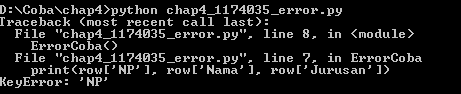
\includegraphics[height=4cm, width=10cm]{figures/4/1174035/Praktek/chap4_1174035_error.png}
	\caption{Contoh KeyError}
	\label{1174035_Error}
\end{figure}
Penanganan : Menggunakan KeyError seperti pada line berikut : \lstinputlisting{src/4/1174035/Praktek/chap4_1174035_error.py}
\begin{figure}[!htbp]
	\centering
	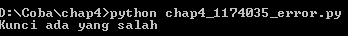
\includegraphics[height=4cm, width=10cm]{figures/4/1174035/Praktek/chap4_1174035_errorfix.png}
	\caption{Hasil Penanganan Error}
	\label{1174035_ErrorFix}
\end{figure}

\section{Hagan Rowlenstino/1174040}
\subsection{Soal 1}
Buatlah fungsi untuk membuka file csv dengan lib csv mode list : 
\lstinputlisting{src/4/1174040/Praktek/1174040_CSV1.py}

\subsection{Soal 2}
Buatlah fungsi untuk membuka file csv dengan lib csv mode dictionary : 
\lstinputlisting{src/4/1174040/Praktek/1174040_CSV2.py}

\subsection{Soal 3}
Buatlah fungsi  untuk membuka file csv dengan lib pandas mode list : 
\lstinputlisting{src/4/1174040/Praktek/1174040_pandas1.py}

\subsection{Soal 4}
Buatlah fungsi  untuk membuka file csv dengan lib pandas mode dictionary : 
\lstinputlisting{src/4/1174040/Praktek/1174040_pandas2.py}

\subsection{Soal 5}
Buatlah fungsi untuk mengubah format tanggal menjadi standard dataframe : 
\lstinputlisting{src/4/1174040/Praktek/1174040_pandas3.py}

\subsection{Soal 6}
Buatlah fungsi  untuk mengubah index kolom : 
\lstinputlisting{src/4/1174040/Praktek/1174040_pandas4.py}

\subsection{Soal 7}
Buatlah fungsi  untuk mengubah atribut atau nama kolom : 
\lstinputlisting{src/4/1174040/Praktek/1174040_pandas5.py}

\subsection{Soal 8}
Disini saya telah membuat file CSV bernama 1174040\_csv.csv untuk di tampilkan, dan sebelum me write ke dalam file csv, terlebih dahulu buat file 1174040\_writecsv.csv : 
\lstinputlisting{src/4/1174040/Praktek/1174040_main.py}

\subsection{Soal 9}
Disini saya telah membuat file CSV bernama 1174040\_csvpandas.csv untuk ditampilkan, dan sebelum me write ke dalam file csv, telebih dahulu buat file 1174040\_writepandas.csv : 
\lstinputlisting{src/4/1174040/Praktek/1174040_main2.py}